%  2.2.3 User Scripting
% -------------------
% TMP scheduler-specific section

The final part of the job script involves the commands that will be executed by the job.
This section should include all necessary commands to set up and run the tasks 
your script is designed to perform. You can use any Linux command in this section, 
ranging from a simple executable call to a complex loop iterating through multiple commands.\\

\noindent \textbf{Best Practice}: prefix any compute-heavy step with \tool{srun}.
This ensures you gain proper insights on the execution of your job.\\

\noindent Each software program may have its own execution framework, as it's the script's author (e.g., you) 
responsibility to review the software's documentation to understand its requirements.
Your script should be written to clearly specify the location of input and output files and the degree of parallelism needed.\\

%
% GE:
%Note that the cluster-specific environment variable, \api{NSLOTS}, resolves 
%to the value provided to the scheduler in the \option{-pe smp} option. 

\noindent Jobs that involve multiple interactions with data input and output files, should make use of \api{TMPDIR}, 
a scheduler-provided workspace nearly 1~TB in size.
\api{TMPDIR} is created on the local disk of the compute node at the start of a job, offering faster I/O operations 
compared to shared storage (provided over NFS).

An sample job script using \api{TMPDIR} is available at \texttt{/home/n/nul-uge/templateTMPDIR.sh}: 
the job is instructed to change to \api{\$TMPDIR}, to make the new directory \texttt{input}, to copy data from
%\texttt{\$SGE\_O\_WORKDIR/references/} to \texttt{input/} (\texttt{\$SGE\_O\_WORKDIR} represents the
\texttt{\$SLURM\_SUBMIT\_DIR/references/} to \texttt{input/} (\texttt{\$SLURM\_SUBMIT\_DIR} represents the
current working directory), to make the new directory \texttt{results}, to
execute the program (which takes input from \texttt{\$TMPDIR/input/} and writes
output to \texttt{\$TMPDIR/results/}), and finally to copy the total end results
to an existing directory, \texttt{processed}, that is located in the current
working directory.
% TODO: verify:
TMPDIR only exists for the duration of the job, though,
so it is very important to copy relevant results from it at job's end.

% -------------- 2.3 Sample Job Script ----------------------
% -----------------------------------------------------------
\subsection{Sample Job Script}
\label{sect:sample-job-script}

Here's a basic job script, \file{tcsh.sh} shown in \xf{fig:tcsh.sh}.
You can copy it from our \href{https://github.com/NAG-DevOps/speed-hpc}{GitHub repository}.

\begin{figure}[htpb]
	\lstinputlisting[language=csh,frame=single,basicstyle=\ttfamily]{tcsh.sh}
	\caption{Source code for \file{tcsh.sh}}
	\label{fig:tcsh.sh}
\end{figure}

\noindent The first line is the shell declaration (also know as a shebang) and sets the shell to \emph{tcsh}.
The lines that begin with \texttt{\#SBATCH} are directives for the scheduler.
%The lines that begin with \texttt{\#\$} are directives for the scheduler.
\begin{itemize}
	%\item \texttt{-N} sets \emph{qsub-test} as the jobname
	\item \texttt{-J} (or \option{--job-name}) sets \emph{tcsh-test} as the job name.
	%\item \texttt{-cwd} tells the scheduler to execute the job from the current working directory
	%\item \texttt{--chdir} tells the scheduler to execute the job from the current working directory
	%\item \texttt{-l h\_vmem=1GB} requests and assigns 1GB of memory to the job. CPU jobs \emph{require} the \texttt{-l h\_vmem} option to be set.
	\item \texttt{--mem=1GB} requests and assigns 1GB of memory to the job. 
	Jobs require the \texttt{--mem} option to be set either in the script
	or on the command line; \textbf{if it's missing, job submission will be rejected.}
\end{itemize}

\noindent The script then:
\begin{enumerate}
	\item Sleeps on a node for 30 seconds.
	\item Uses the \tool{module} command to load the \texttt{gurobi/8.1.0} environment.
	\item Prints the list of loaded modules into a file.
\end{enumerate}

%The scheduler command, \tool{qsub}, is used to submit (non-interactive) jobs. 
\noindent The scheduler command, \tool{sbatch}, is used to submit (non-interactive) jobs. 
%From an ssh session on speed-submit, submit this job with \texttt{qsub ./tcsh.sh}.
From an ssh session on ``speed-submit'', submit this job with
\begin{verbatim}
    sbatch ./tcsh.sh
\end{verbatim}

%You will see, \texttt{"Your job X ("qsub-test") has been submitted"}.
\noindent You will see, \texttt{Submitted batch job 2653} where $2653$ is a job ID assigned.
%The command, \tool{qstat}, can be used 
The commands, \tool{squeue} and \tool{sinfo} can be used 
%to look at the status of the cluster: \texttt{qstat -f -u "*"}.
to look at the status of the cluster: \texttt{squeue -l}.

%\small
%\begin{verbatim}
%queuename                      qtype resv/used/tot. load_avg arch          states
%---------------------------------------------------------------------------------
%a.q@speed-01.encs.concordia.ca BIP   0/0/32         0.01     lx-amd64
%---------------------------------------------------------------------------------
%a.q@speed-03.encs.concordia.ca BIP   0/0/32         0.01     lx-amd64
%---------------------------------------------------------------------------------
%a.q@speed-25.encs.concordia.ca BIP   0/0/32         0.01     lx-amd64
%---------------------------------------------------------------------------------
%a.q@speed-27.encs.concordia.ca BIP   0/0/32         0.01     lx-amd64
%---------------------------------------------------------------------------------
%g.q@speed-05.encs.concordia.ca BIP   0/0/32         0.02     lx-amd64
     %144   100.00000 qsub-test nul-uge     r     12/03/2018 16:39:30    1 
     %62624 0.09843 case_talle x_yzabc      r     11/09/2021 16:50:09    32
%---------------------------------------------------------------------------------
%g.q@speed-17.encs.concordia.ca BIP   0/0/32         0.01     lx-amd64
%---------------------------------------------------------------------------------
%s.q@speed-07.encs.concordia.ca BIP   0/0/32         0.04     lx-amd64
%---------------------------------------------------------------------------------
%s.q@speed-08.encs.concordia.ca BIP   0/0/32         0.01     lx-amd64
%---------------------------------------------------------------------------------
%s.q@speed-09.encs.concordia.ca BIP   0/0/32         0.01     lx-amd64
%---------------------------------------------------------------------------------
%s.q@speed-10.encs.concordia.ca BIP   0/32/32        32.72    lx-amd64
     %62624 0.09843 case_talle x_yzabc      r     11/09/2021 16:50:09    32
%---------------------------------------------------------------------------------
%s.q@speed-11.encs.concordia.ca BIP   0/32/32        32.08    lx-amd64
     %62679 0.14212 CWLR_DF    a_bcdef      r     11/10/2021 17:25:19    32
%---------------------------------------------------------------------------------
%s.q@speed-12.encs.concordia.ca BIP   0/32/32        32.10    lx-amd64
     %62749 0.09000 CLOUDY     z_abc        r     11/11/2021 21:58:12    32
%---------------------------------------------------------------------------------
%s.q@speed-15.encs.concordia.ca BIP   0/4/32         0.03     lx-amd64
     %62753 82.47478 matlabLDPa b_bpxez      r     11/12/2021 08:49:52     4
%---------------------------------------------------------------------------------
%s.q@speed-16.encs.concordia.ca BIP   0/32/32        32.31    lx-amd64
     %62751 0.09000 CLOUDY     z_abc        r     11/12/2021 06:03:54    32
%---------------------------------------------------------------------------------
%s.q@speed-19.encs.concordia.ca BIP   0/32/32        32.22    lx-amd64
%---------------------------------------------------------------------------------
%...
%---------------------------------------------------------------------------------
%s.q@speed-35.encs.concordia.ca BIP   0/32/32        2.78     lx-amd64
     %62754 7.22952 qlogin-tes a_tiyuu      r     11/12/2021 10:31:06    32
%---------------------------------------------------------------------------------
%s.q@speed-36.encs.concordia.ca BIP   0/0/32         0.03     lx-amd64
%etc.

\small
\begin{verbatim}
[serguei@speed-submit src] % squeue -l
Thu Oct 19 11:38:54 2023
JOBID PARTITION     NAME     USER    STATE       TIME TIME_LIMI  NODES NODELIST(REASON)
 2641        ps interact   b_user  RUNNING   19:16:09 1-00:00:00      1 speed-07
 2652        ps interact   a_user  RUNNING      41:40 1-00:00:00      1 speed-07
 2654        ps tcsh-tes  serguei  RUNNING       0:01 7-00:00:00      1 speed-07
[serguei@speed-submit src] % sinfo
PARTITION AVAIL  TIMELIMIT  NODES  STATE NODELIST
ps*          up 7-00:00:00     14  drain speed-[08-10,12,15-16,20-22,30-32,35-36]
ps*          up 7-00:00:00      1    mix speed-07
ps*          up 7-00:00:00      7   idle speed-[11,19,23-24,29,33-34]
pg           up 1-00:00:00      1  drain speed-17
pg           up 1-00:00:00      3   idle speed-[05,25,27]
pt           up 7-00:00:00      7   idle speed-[37-43]
pa           up 7-00:00:00      4   idle speed-[01,03,25,27]
\end{verbatim}
\normalsize

\noindent \textbf{Remember} that you only have 30 seconds before the job is essentially over, so 
if you do not see a similar output, either adjust the sleep time in the 
%script, or execute the \tool{qstat} statement more quickly. The \tool{qstat} 
script, or execute the \tool{sbatch} statement more quickly. The \tool{squeue} 
output listed above shows that your job 2654 is running on node \texttt{speed-07}, 
and its time limit is 7 days, etc.\\
% TODO
%, that it 
%was started at 16:39:30 on 12/03/2018, and that it is a single-core job (the 
%default). 

Once the job finishes, there will be a new file in the directory that the job 
%was started from, with the syntax of, \texttt{"job name".o"job number"}, so 
was started from, with the syntax of, \texttt{slurm-<job id>.out}, so 
%in this example the file is, qsub \file{test.o144}. This file represents the 
in this example the file is, \file{slurm-2654.out}. This file represents the 
standard output (and error, if there is any) of the job in question. If you 
look at the contents of your newly created file, you will see that it 
contains the output of the, \texttt{module list} command. 
Important information is often written to this file.
%
%Congratulations on your first job! 

% -------------- 2.4 Common Job Management Commands Summary ---
% -------------------------------------------------------------
\subsection{Common Job Management Commands Summary}
\label{sect:job-management-commands}

Here is a summary of useful job management commands for handling various aspects of 
job submission and monitoring on the Speed cluster:

\begin{itemize}
	\item Submitting a job:
	\begin{verbatim}
		sbatch -A <ACCOUNT> -t <MINUTES> --mem=<MEMORY> -p <PARTITION> ./<myscript>.sh
	\end{verbatim}

	\item Checking your job(s) status:
	\begin{verbatim}
		squeue -u <ENCSusername>
	\end{verbatim}

	\item Displaying cluster status:
	\begin{verbatim}
		squeue
	\end{verbatim}
		\begin{itemize}
			\item Use \option{-A} for per account (e.g., \texttt{-A vidpro}, \texttt{-A aits}), 
			\item Use \option{-p} for per partition (e.g., \texttt{-p ps}, \texttt{-p pg}, \texttt{-p pt}), etc.
		\end{itemize}

	\item Displaying job information:
	\begin{verbatim}
		squeue --job <job-ID>
	\end{verbatim}

	\item Displaying individual job steps: (to see which step failed if you used \tool{srun})
	\begin{verbatim}
		squeue -las
	\end{verbatim}

	\item Monitoring job and cluster status: (view \tool{sinfo} and watch the queue for your job(s))
	\begin{verbatim}
		watch -n 1 "sinfo -Nel -pps,pt,pg,pa && squeue -la"
	\end{verbatim}

	\item Canceling a job:
	\begin{verbatim}
		scancel <job-ID>
	\end{verbatim}

	\item Holding a job:
	\begin{verbatim}
		scontrol hold <job-ID>
	\end{verbatim}

	\item Releasing a job:
	\begin{verbatim}
		scontrol release <job-ID>
	\end{verbatim}

	\item Getting job statistics: (including useful metrics like ``maxvmem'')
	\begin{verbatim}
		sacct -j <job-ID>
	\end{verbatim}
	
	\api{maxvmem} is one of the more useful stats that you can elect to display
	as a format option.
	\small
	\begin{verbatim}
	% sacct -j 2654
	JobID           JobName  Partition    Account  AllocCPUS      State ExitCode
	------------ ---------- ---------- ---------- ---------- ---------- --------
	2654          tcsh-test         ps     speed1          1  COMPLETED      0:0
	2654.batch        batch                speed1          1  COMPLETED      0:0
	2654.extern      extern                speed1          1  COMPLETED      0:0
	% sacct -j 2654 -o jobid,user,account,MaxVMSize,Reason%10,TRESUsageOutMax%30
	JobID             User    Account  MaxVMSize     Reason        TRESUsageOutMax
	------------ --------- ---------- ---------- ---------- ----------------------
	2654           serguei     speed1                  None
	2654.batch                 speed1    296840K             energy=0,fs/disk=1975
	2654.extern                speed1    296312K              energy=0,fs/disk=343
	\end{verbatim}
	\normalsize
	See \texttt{man sacct} or \texttt{sacct -e} for details of the available formatting options. 
	You can define your preferred default format in the \api{SACCT\_FORMAT} environment variable
	in your \texttt{.cshrc} or \texttt{.bashrc} files.

	\item Displaying job efficiency: (including cpu and memory utilization)\\
	\texttt{seff <job-ID>}\\
	Don't execute it on RUNNING jobs (only on completed/finished jobs), efficiency statistics may be misleading.
	If you define the following directive in your batch script, your ENCS email address will receive an email with seff output when your job is finished.
	\begin{verbatim}
	#SBATCH --mail-type=ALL        
	\end{verbatim}

	Output example:
	\small
	\begin{verbatim}
	Job ID: XXXXX
	Cluster: speed
	User/Group: user1/user1
	State: COMPLETED (exit code 0)
	Nodes: 1
	Cores per node: 4
	CPU Utilized: 00:04:29
	CPU Efficiency: 0.35% of 21:32:20 core-walltime
	Job Wall-clock time: 05:23:05
	Memory Utilized: 2.90 GB
	Memory Efficiency: 2.90% of 100.00 GB
	\end{verbatim}
	\normalsize
\end{itemize}

%\begin{itemize}
	%\item
	%\texttt{qsub ./<myscript>.sh}: once that your job script is ready,
	%on \texttt{speed-submit} you can submit it using this
	%\item
	%\texttt{qstat -f -u <ENCSusername>}: you can check the status of your job(s)
	%\item
	%\texttt{qstat -f -u "*"}: display cluster status for all users. 
	%\item
	%\texttt{qstat -j [job-ID]}: display job information for [job-ID] (said job may be actually running, or waiting in the queue). 
	%\item
	%\texttt{qdel [job-ID]}: delete job [job-ID]. 
	%item
	%\texttt{qhold [job-ID]}: hold queued job, [job-ID], from running.
	%item
	%\texttt{qrls [job-ID]}: release held job [job-ID]. 
%\end{itemize}

% -------------- 2.5 Advanced sbatch Options ------------------
% -------------------------------------------------------------
%\subsection{Advanced \tool{qsub} Options}
\subsection{Advanced \tool{sbatch} Options}
\label{sect:submit-options}
\label{sect:qsub-options}

In addition to the basic sbatch options presented earlier, 
there are several advanced options that are generally useful:

\begin{itemize}
	%\texttt{-m bea}: requests that the scheduler e-mail you when a job (b)egins;
	%(e)nds; (a)borts. Mail is sent to the default address of,
	%\texttt{"username@encs.concordia.ca"}, unless a different address is supplied (see, 
	%\texttt{-M}). The report sent when a job ends includes job 
	%runtime, as well as the maximum memory value hit (\api{maxvmem}). 
	\item E-mail notifications:
	\begin{verbatim}
		--mail-type=<TYPE>
	\end{verbatim}
	Requests the scheduler to send an email when the job changes state.
	\texttt{<TYPE>} can be \texttt{ALL}, \texttt{BEGIN}, \texttt{END}, or \texttt{FAIL}.
	Mail is sent to the default address of, \texttt{"<ENCSusername>@encs.concordia.ca"}, 
	which you can consult via \texttt{webmail.encs} unless a different address is supplied 
	(see, \texttt{--mail-user}).
	% TODO: double-check
	The report sent when a job ends includes job 
	runtime, as well as the maximum memory value hit (\api{maxvmem}). 
	\begin{verbatim}
		--mail-user email@domain.com
	\end{verbatim}
	Specifies a different email address for notifications rather than the default.
	%\texttt{-M email@domain.com}: requests that the scheduler use this e-mail 
	%notification address, rather than the default (see, \texttt{-m}). 

	\item Export environment variables used by the script.:
	\begin{verbatim}
		--export=ALL
		--export=NONE
		--export=VARIABLES
	\end{verbatim}
	%\texttt{-v variable[=value]}: exports an environment variable that can be used by the script.

	\item Job runtime:
	%\texttt{-l h\_rt=[hour]:[min]:[sec]}: sets a job runtime of HH:MM:SS. Note 
	%that if you give a single number, that represents \emph{seconds}, not hours.
	\begin{verbatim}
		-t <MINUTES> or DAYS-HH:MM:SS
	\end{verbatim} 
	sets a job runtime of min or HH:MM:SS. Note that if you give a single number, that represents \emph{minutes}, not hours. 

	\item Job Dependencies:
	%\texttt{-hold\_jid [job-ID]}: run this job only when job [job-ID] finishes. Held jobs appear in the queue. 
	\begin{verbatim}
		--depend=<state:job-ID>
	\end{verbatim} 
	Runs the job only when the specified job <job-ID> finishes. This is useful for creating job chains where 
	subsequent jobs depend on the completion of previous ones.
\end{itemize}

\noindent \textbf{Note:} \tool{sbatch} options can be specified during the job-submission 
command, and these \emph{override} existing script options (if present). The 
syntax is
\begin{verbatim}
	sbatch [options] PATHTOSCRIPT
\end{verbatim}
but unlike in the script, the options are specified without the leading \verb+#SBATCH+
e.g.: 
\begin{verbatim}
	sbatch -J sub-test --chdir=./ --mem=1G ./tcsh.sh
\end{verbatim}

% -------------- 2.6 Array Jobs -------------------------------
% -------------------------------------------------------------
\subsection{Array Jobs}
\label{sect:array-jobs}

Array jobs are those that start a batch job or a parallel job multiple times. 
Each iteration of the job array is called a task and receives a unique job ID.
Array jobs are particularly useful for running a large number of similar tasks with slight variations.\\

%To submit an array job, use the \texttt{\-t} option of the \texttt{qsub} 
%command as follows:
\noindent To submit an array job (Only supported for batch jobs), use the \option{--array} option of the \texttt{sbatch} 
command as follows:

%\begin{verbatim}
%qsub -t n[-m[:s]] <batch_script>
%\end{verbatim}
\begin{verbatim}
	sbatch --array=n-m[:s]] <batch_script>
\end{verbatim}

\noindent \textbf{where}
\begin{itemize}
	\item
	\texttt{n}: indicates the start-id.
	\item
	\texttt{m}: indicates the max-id.
	\item
	\texttt{s}: indicates the step size.
\end{itemize}

\noindent \textbf{Examples:}
\begin{itemize}
	\item Submit a job with 1 task where the task-id is 10. 
	%\texttt{qsub -t 10 array.sh}: submits a job with 1 task where the task-id is 10. 
	\begin{verbatim}
		sbatch --array=10 array.sh
	\end{verbatim}

	\item Submit a job with 10 tasks numbered consecutively from 1 to 10.
	%\texttt{qsub -t 10 array.sh}: submits a job with 1 task where the task-id is 10. 
	\begin{verbatim}
		sbatch --array=1-10 array.sh
	\end{verbatim}

	\item Submit a job with 5 tasks numbered consecutively with a step size of 3 (task-ids 3,6,9,12,15)
	%\texttt{qsub -t 3-15:3 array.sh}: submits a jobs with 5 tasks numbered consecutively with step size 3
	\begin{verbatim}
		sbatch --array=3-15:3 array.sh
	\end{verbatim}

	\item Submit a job with 50000 elements, where \%a maps to the task-id between 1 and 50K. 
	\begin{verbatim}
		sbatch --array=1-50000 -N1 -i my_in_%a -o my_out_%a array.sh
	\end{verbatim}
\end{itemize}

\noindent \textbf{Output files for Array Jobs:}\\
The default output and error-files are \texttt{slurm-job\_id\_task\_id.out}.
%\option{job\_name.[o|e]job\_id} and\\
%\option{job\_name.[o|e]job\_id.task\_id}.
%
This means that Speed creates an output and an error-file for each task 
generated by the array-job, as well as one for the super-ordinate array-job. 
To alter this behavior use the \option{-o} and \option{-e} options of \tool{sbatch}.\\
%\tool{qsub}. 

For more details about Array Job options, please review the manual pages for 
%\option{qsub} by executing the following at the command line on speed-submit 
%\tool{man qsub}.
\tool{sbatch} by executing the following at the command line on \tool{speed-submit }
\texttt{man sbatch}.
 
% -------------- 2.7 Requesting Multiple Cores ----------------
% -------------------------------------------------------------
\subsection{Requesting Multiple Cores (i.e., Multithreading Jobs)}
\label{sect:multicore-jobs}

For jobs that can take advantage of multiple machine cores, you can 
request up to 32 cores (per job) in your script using the following options:

%\begin{verbatim}
%#$ -pe smp [#cores] 
%\end{verbatim}
\begin{verbatim}
	#SBATCH -n <#cores for processes>
	#SBATCH -n 1
	#SBATCH -c <#cores for threads of a single process>
\end{verbatim}

\noindent Both \tool{sbatch} and \tool{salloc} support \option{-n} on the command line,
and it should always be used either in the script or on the command line as the
default $n=1$.\\

\noindent \textbf{Important Considerations}:
\begin{itemize}
	\item Do not request more cores than you think will be useful, 
	as larger-core jobs are more difficult to schedule.

	\item If you are running a program that scales out to the maximum single-machine 
	core count available, please request 32 cores to avoid node 
	oversubscription (i.e., overloading the CPUs).
\end{itemize}

\noindent \textbf{Note:} \option{--ntasks} or \option{--ntasks-per-node}
(\option{-n}) refers to processes (usually the ones run with \tool{srun}).
\option{--cpus-per-task} (\option{-c}) corresponds to threads per process.\\

\noindent Some programs consider them equivalent, while others do not. For example, 
Fluent uses \option{--ntasks-per-node=8} and \option{--cpus-per-task=1},
whereas others may set \option{--cpus-per-task=8} and \option{--ntasks-per-node=1}.
If one of these is not 1, some applications need to be configured to use n * c total cores.\\

\noindent Core count associated with a job appears under,
%``states'', in the, \texttt{qstat -f -u "*"}, output.
``AllocCPUS'', in the, \texttt{sacct -j <job-id>}, output.

\small
\begin{verbatim}
	[serguei@speed-submit src] % squeue -l
	Thu Oct 19 20:32:32 2023
	JOBID PARTITION     NAME     USER    STATE       TIME TIME_LIMI  NODES NODELIST(REASON)
	2652        ps interact   a_user  RUNNING   9:35:18 1-00:00:00      1 speed-07
	[serguei@speed-submit src] % sacct -j 2652
	JobID           JobName  Partition    Account  AllocCPUS      State ExitCode
	------------ ---------- ---------- ---------- ---------- ---------- --------
	2652         interacti+         ps     speed1         20    RUNNING      0:0
	2652.intera+ interacti+                speed1         20    RUNNING      0:0
	2652.extern      extern                speed1         20    RUNNING      0:0
	2652.0       gydra_pmi+                speed1         20  COMPLETED      0:0
	2652.1       gydra_pmi+                speed1         20  COMPLETED      0:0
	2652.2       gydra_pmi+                speed1         20     FAILED      7:0
	2652.3       gydra_pmi+                speed1         20     FAILED      7:0
	2652.4       gydra_pmi+                speed1         20  COMPLETED      0:0
	2652.5       gydra_pmi+                speed1         20  COMPLETED      0:0
	2652.6       gydra_pmi+                speed1         20  COMPLETED      0:0
	2652.7       gydra_pmi+                speed1         20  COMPLETED      0:0
\end{verbatim}
\normalsize

% -------------- 2.8 Interactive Jobs -------------------------
% -------------------------------------------------------------
\subsection{Interactive Jobs}
\label{sect:interactive-jobs}

Interactive job sessions allow you to interact with the system in real-time. 
These sessions are particularly useful for tasks such as testing, debugging, optimizing code, 
setting up environments, and other preparatory work before submitting batch jobs.

%  2.8.1 Command Line
% -------------------
\subsubsection{Command Line}
\label{sect:command-line}

To request an interactive job session, use the \texttt{salloc} command with appropriate options.
This is similar to submitting a batch job but allows you to run shell commands interactively 
within the allocated resources. For example:
\begin{verbatim}
	salloc -J interactive-test --mem=1G -p ps -n 8
\end{verbatim}

\noindent Within the allocated \tool{salloc} session, you can run shell commands as usual. 
It is recommended to use \tool{srun} for compute-intensive steps within \tool{salloc}. 
If you need a quick, short job just to compile something on a GPU node, 
you can use an interactive srun directly. For example, a 1-hour allocation:

\noindent \textbf{For tcsh}:
\begin{verbatim}
	srun --pty -n 8 -p pg --gpus=1 --mem=1Gb -t 60 /encs/bin/tcsh
\end{verbatim}

\noindent \textbf{For bash}:
\begin{verbatim}
	srun --pty -n 8 -p pg --gpus=1 --mem=1Gb -t 60 /encs/bin/bash
\end{verbatim}

%session, use, \texttt{qlogin [options]}, similarly to a 
%\tool{qsub} command-line job (e.g., \texttt{qlogin -N qlogin-test -l h\_vmem=1G}).
%Note that the options that are available for \tool{qsub} are not necessarily
%available for \tool{qlogin}, notably, \texttt{-cwd}, and, \texttt{-v}. 

%  2.8.2 Graphical Applications
% -------------------
\subsubsection{Graphical Applications}
\label{sect:graphical-applications}

To run graphical UI applications (e.g., MALTLAB, Abaqus CME, IDEs like PyCharm, VSCode, Eclipse, etc.) on Speed, 
you need to enable X11 forwarding from your client machine Speed then to the compute node.
To do so, follow these steps:

\begin{enumerate}
	\item Run an X server on your client machine:
	\begin{itemize}
		\item \textbf{Windows:} Use MobaXterm with X turned on, or Xming + PuTTY with X11 forwarding, or XOrg under Cygwin
		\item \textbf{macOS:} Use XQuarz -- use its \tool{xterm} and \texttt{ssh -X}
		\item \textbf{Linux:} Use \texttt{ssh -X speed.encs.concordia.ca}
	\end{itemize}
	For more details, see \href{https://www.concordia.ca/ginacody/aits/support/faq/xserver.html}{How do I remotely launch X(Graphical) applications?}

	\item Verify that X11 forwarding is enabled by printing the \api{DISPLAY} variable:
	\begin{verbatim}
		echo $DISPLAY
	\end{verbatim}

	\item Start an interactive session with X11 forwarding enabled (Use the \option{--x11} with \tool{salloc} or \tool{srun}), for example:
	\begin{verbatim}
		salloc -p ps --x11=first --mem=4Gb -t 0-06:00
	\end{verbatim}

	\item Once landed on a compute node, verify \api{DISPLAY} again.
	
	\item Set the \api{XDG\_RUNTIME\_DIR} variable to a directory in your \tool{speed-scratch} space:
	\begin{verbatim}
		mkdir -p /speed-scratch/$USER/run-dir
		setenv XDG_RUNTIME_DIR /speed-scratch/$USER/run-dir
	\end{verbatim}
	
	\item Launch your graphical application:
	\begin{verbatim}
		module load matlab/R2023a/default 
		matlab
	\end{verbatim}
\end{enumerate}

\noindent Here's an example of starting PyCharm (see \xf{fig:pycharm}). 
\textbf{Note:} If using VSCode, it's currently only supported with the \tool{--no-sandbox} option.\\

\small
\noindent \textbf{TCSH version:}
\begin{verbatim}
	ssh -X speed (XQuartz xterm, PuTTY or MobaXterm have X11 forwarding too)
	[speed-submit] [/home/c/carlos] > echo $DISPLAY
	localhost:14.0
	[speed-submit] [/home/c/carlos] > cd /speed-scratch/$USER
	[speed-submit] [/speed-scratch/carlos] > echo $DISPLAY
	localhost:13.0
	[speed-submit] [/speed-scratch/carlos] > salloc -pps --x11=first --mem=4Gb -t 0-06:00
	[speed-07] [/speed-scratch/carlos] > echo $DISPLAY
	localhost:42.0
	[speed-07] [/speed-scratch/carlos] > hostname
	speed-07.encs.concordia.ca
	[speed-07] [/speed-scratch/carlos] > setenv XDG_RUNTIME_DIR /speed-scratch/$USER/run-dir
	[speed-07] [/speed-scratch/carlos] > /speed-scratch/nag-public/bin/pycharm.sh
\end{verbatim}

\noindent \textbf{BASH version:}
\begin{verbatim}
	bash-3.2$ ssh -X speed (XQuartz xterm, PuTTY or MobaXterm have X11 forwarding too)
	serguei@speed's password: 
	[serguei@speed-submit ~] % echo $DISPLAY
	localhost:14.0
	[serguei@speed-submit ~] % salloc -p ps --x11=first --mem=4Gb -t 0-06:00 
	bash-4.4$ echo $DISPLAY
	localhost:77.0
	bash-4.4$ hostname
	speed-01.encs.concordia.ca
	bash-4.4$ export XDG_RUNTIME_DIR=/speed-scratch/$USER/run-dir
	bash-4.4$ /speed-scratch/nag-public/bin/pycharm.sh
	\end{verbatim}
\normalsize

\begin{figure}[htpb]
	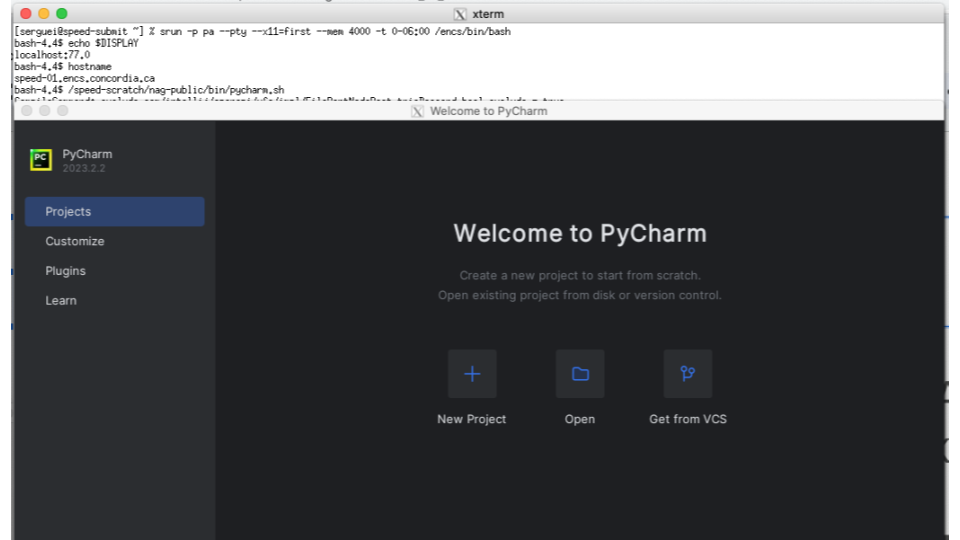
\includegraphics[width=\columnwidth]{images/pycharm}
	\caption{Launching PyCharm on a Speed Node}
	\label{fig:pycharm}
\end{figure}

%  2.8.3 Jupyter Notebooks in Singularity
% -------------------
\subsubsection{Jupyter Notebook in Singularity}
\label{sect:jupyter}

To run Jupyter Notebooks using Singularity (more on Singularity see \xs{sect:singularity-containers}), follow these steps:
% Here we are using one of the OpenISS-derived containers (see \xs{sect:openiss-examples} as well).

\begin{enumerate}
	\item Connect to Speed with X11 forwarding enabled:
	\item Use the \option{--x11} with \tool{salloc} or \tool{srun} as described in the above example
	\item Load Singularity module
		\verb+module load singularity/3.10.4/default+

	\item Execute this Singularity command on a single line. or save it in a shell script where you could easily call it.
	\small
	\begin{verbatim}
		srun singularity exec -B $PWD\:/speed-pwd,/speed-scratch/$USER\:/my-speed-scratch,/nettemp \
		--env SHELL=/bin/bash --nv /speed-scratch/nag-public/openiss-cuda-conda-jupyter.sif \
		/bin/bash -c '/opt/conda/bin/jupyter notebook --no-browser --notebook-dir=/speed-pwd \
		--ip="*" --port=8888 --allow-root'
	\end{verbatim}
	\normalsize

	\item In a new terminal window, create an \tool{ssh} tunnel between your computer and the node (\texttt{speed-XX}) where Jupyter is
	running (Using \texttt{speed-submit} as a ``jump server'') (Preferably: PuTTY, see \xf{fig:putty1} and \xf{fig:putty2})
	\begin{verbatim}
		ssh -L 8888:speed-XX:8888 <ENCS-username>@speed-submit.encs.concordia.ca
	\end{verbatim}
	Don't close the tunnel.

	\item Open a browser, and copy your Jupyter's token (it printed to you in the terminal) and paste it in the browser's URL field.
	In our case, the URL is:
	\begin{verbatim}
		http://localhost:8888/?token=5a52e6c0c7dfc111008a803e5303371ed0462d3d547ac3fb
	\end{verbatim}

	\item Access the Jupyter Notebook interface in your browser.
\end{enumerate}

\begin{figure}[htbp]
	\centering
	\fbox{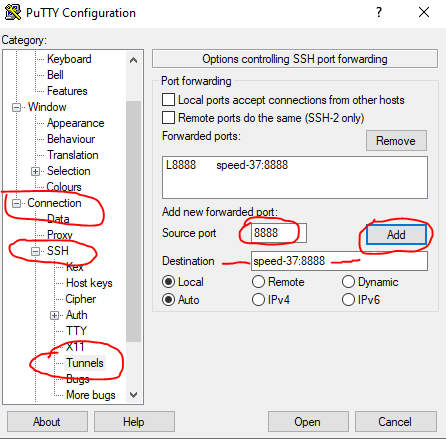
\includegraphics{images/putty1}}
	\caption{SSH tunnel configuration 1}
	\label{fig:putty1}
\end{figure}

\begin{figure}[htbp]
	\centering
	\fbox{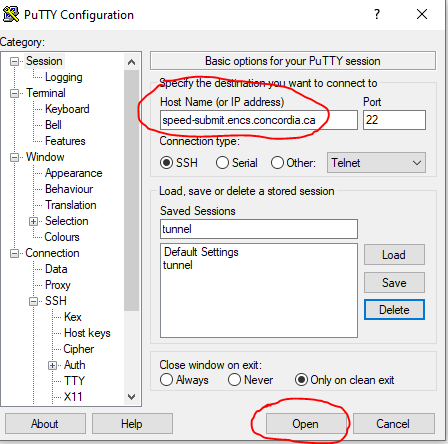
\includegraphics{images/putty2}}
	\caption{SSH tunnel configuration 2}
	\label{fig:putty2}
\end{figure}

\begin{figure}[htbp]
	\centering
	\fbox{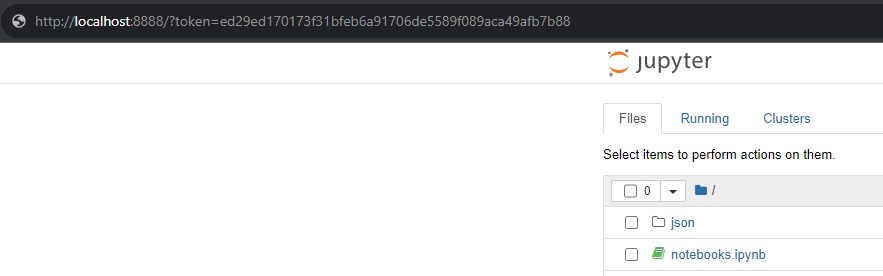
\includegraphics[width=1.00\textwidth]{images/jupyter.png}}
	\caption{Jupyter running on a Speed node}
	\label{fig:jupyter}
\end{figure}

%  2.8.4 JupyterLab in Conda and Pytorch
% -------------------
\subsubsection{JupyterLab in Conda and Pytorch}
\label{sect:jupiterlabs}

For setting up Jupyter Labs with Conda and Pytorch, follow these steps:

\begin{itemize}
	\item Environment preparation: (only once, takes some time to run to install all things)
	\begin{enumerate}
		\item Navigate to your speed-scratch directory:
		\begin{verbatim}
			cd /speed-scratch/\$USER
		\end{verbatim}

		\item Create a Jupyter (name of your choice) directory and cd into it: \texttt{mkdir -p Jupyter}
		\begin{verbatim}
			mkdir -p Jupyter
			cd Jupyter
		\end{verbatim}

		\item Start an interactive session:
		\begin{verbatim}
			salloc --mem=50G --gpus=1 -ppg (or -ppt)
		\end{verbatim}
		
		\item Set conda environment variables, amd install jupyterlab and pytorch:
		\small
		\begin{verbatim}
			module load anaconda3/2023.03/default
			setenv TMPDIR /speed-scratch/$USER/tmp
			setenv TMP /speed-scratch/$USER/tmp
			setenv CONDA_PKGS_DIRS /speed-scratch/$USER/Jupyter/pkgs 
			conda create -p /speed-scratch/$USER/Jupyter/jupyter-env 
			conda activate /speed-scratch/$USER/Jupyter/jupyter-env
			conda install -c conda-forge jupyterlab
			pip3 install torch torchvision torchaudio --index-url https://download.pytorch.org/whl/cu118
			exit
		\end{verbatim}
		\normalsize
	\end{enumerate}

	\item Execution of Jupyter Labs from \textbf{speed-submit} (Repeat this every time you want to run Jupyter Labs):
	\begin{enumerate}
		\item Open an Interactive session: \texttt{salloc --mem=50G --gpus=1 -ppg} (or -ppt)
		\item Start an interactive session:
		\begin{verbatim}
			salloc --mem=50G --gpus=1 -ppg (or -ppt)
		\end{verbatim}

		\item Activate conda environment and run Jupyter Labs:
		\begin{verbatim}
			cd /speed-scratch/$USER/Jupyter
			module load anaconda3/2023.03/default
			setenv TMPDIR /speed-scratch/$USER/tmp
			setenv TMP /speed-scratch/$USER/tmp
			setenv CONDA_PKGS_DIRS /speed-scratch/$USER/Jupyter/pkgs
			conda activate /speed-scratch/$USER/Jupyter/jupyter-env
			jupyter lab --no-browser --notebook-dir=$PWD --ip="*" --port=8888 --port-retries=50
		\end{verbatim}

		\item Verify which port the system has assigned to Jupyter: \texttt{http://localhost:XXXX/lab?token=}
		\item In a new terminal window, create an \tool{ssh} tunnel similar to Jupyter in Singularity, see \xs{sect:jupyter}
		\item Open a browser and copy your Jupyter's token and paste it in the browser's URL field
	\end{enumerate}
\end{itemize}

%  2.8.5 JupyterLab + Pytorch in Python venv
% -------------------
\subsubsection{JupyterLab + Pytorch in Python venv}
\label{sect:jupiterlabs-venv}

This is an example of Jupyter Labs running in a Python Virtual environment (venv), with Pytorch

\begin{itemize}
\item
Environment preparation: for the FIRST time:
\begin{enumerate}
\item
Go to your speed-scratch directory: \texttt{cd /speed-scratch/\$USER}
\item
Open an Interactive session: \texttt{salloc --mem=50G --gpus=1 --constraint=el9}
\item
Create Python venv and install jupyterlab+pytorch
\scriptsize
\begin{verbatim}
module load python/3.11.5/default
setenv TMPDIR /speed-scratch/$USER/tmp
setenv TMP /speed-scratch/$USER/tmp
setenv PIP_CACHE_DIR /speed-scratch/$USER/tmp/cache
python -m venv /speed-scratch/$USER/tmp/jupyter-venv
source /speed-scratch/$USER/tmp/jupyter-venv/bin/activate.csh
pip install jupyterlab
pip3 install torch torchvision torchaudio --index-url https://download.pytorch.org/whl/cu118
exit
\end{verbatim}
\normalsize
\end{enumerate}
\item
Running Jupyter Labs, from \textbf{speed-submit}:
\begin{enumerate}
\item
Open an Interactive session: \texttt{salloc --mem=50G --gpus=1 --constraint=el9} 
\scriptsize
\begin{verbatim}
cd /speed-scratch/$USER
module load python/3.11.5/default
setenv PIP_CACHE_DIR /speed-scratch/$USER/tmp/cache
source /speed-scratch/$USER/tmp/jupyter-venv/bin/activate.csh
jupyter lab --no-browser --notebook-dir=$PWD --ip="0.0.0.0" --port=8888 --port-retries=50
\end{verbatim}
\normalsize
\item
Verify which port the system has assigned to Jupyter: 
\texttt{http://localhost:XXXX/lab?token=}
\item
SSH Tunnel creation: similar to Jupyter in Singularity, see \xs{sect:jupyter}
\item
Open a browser and type: \texttt {localhost:XXXX} (port assigned)
\end{enumerate}
\end{itemize}


% ------------------------------------------------------------------------------
\subsubsection{VScode}
\label{sect:vscode}

This is an example of running VScode, it's similar to Jupyter notebooks, but it doesn't use containers.
This a Web version, it exists the local(workstation)-remote(speed-node) version too, but it is for Advanced users (no support, execute it at your own risk).

\begin{itemize}
\item
Environment preparation: for the FIRST time:
\begin{enumerate}
\item
Go to your speed-scratch directory: \texttt{cd /speed-scratch/\$USER}
\item
Create a vscode directory: \texttt{mkdir vscode}
\item
Go to vscode: \texttt{cd vscode}
\item
Create home and projects: \texttt{mkdir \{home,projects\}}
\item
Create this directory: \texttt {mkdir -p /speed-scratch/\$USER/run-user}
\end{enumerate}
\item
Running VScode
\begin{enumerate}
\item 
Go to your vscode directory: \texttt{cd /speed-scratch/\$USER/vscode}
\item
Open interactive session: \texttt {salloc --mem=10Gb --constraint=el9}
\item
Set environment variable: \texttt {setenv XDG\_RUNTIME\_DIR /speed-scratch/\$USER/run-user}
\item 
Run VScode, change the port if needed.
\scriptsize
\begin{verbatim}
/speed-scratch/nag-public/code-server-4.22.1/bin/code-server --user-data-dir=$PWD\/projects \
--config=$PWD\/home/.config/code-server/config.yaml --bind-addr="0.0.0.0:8080" $PWD\/projects
\end{verbatim}
\normalsize
\item
SSH Tunnel creation: similar to Jupyter, see \xs{sect:jupyter}
\item
Open a browser and type: \texttt {localhost:8080}
\item
If the browser asks for password: 
\begin{verbatim}
cat /speed-scratch/$USER/vscode/home/.config/code-server/config.yaml
\end{verbatim}

\end{enumerate}
\end{itemize}

\begin{figure}[htbp]
	\centering
	\fbox{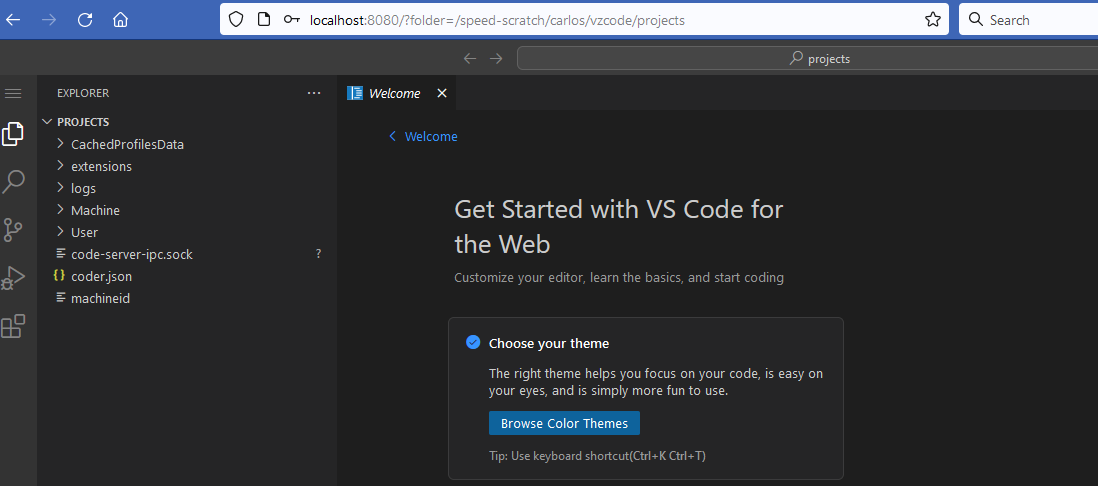
\includegraphics[width=1.00\textwidth]{images/vscode.png}}
	\caption{VScode running on a Speed node}
	\label{fig:vscode}
\end{figure}

% ------------------------------------------------------------------------------
\subsection{Scheduler Environment Variables}
\label{sect:env-vars}

The scheduler presents a number of environment variables that can be used in 
your jobs. You can invoke \tool{env} or \tool{printenv} in your
job to know what hose are (most begin with the prefix \texttt{SLURM}).
%
Some of the more useful ones are:
%\api{TMPDIR}, \api{SGE\_O\_WORKDIR}, and \api{NSLOTS}:

\begin{itemize}
\item
% TODO: verify temporal existence
\api{\$TMPDIR} -- the path to the job's temporary space on the node. It
\emph{only} exists for the duration of the job, so if data in the temporary space 
are important, they absolutely need to be accessed before the job terminates.

%\item
%\api{\$SGE\_O\_WORKDIR}=the path to the job's working directory (likely an
%NFS-mounted path). If, \texttt{-cwd}, was stipulated, that path is taken; if not, 
%the path defaults to your home directory.
\item
\api{\$SLURM\_SUBMIT\_DIR} -- the path to the job's working directory (likely an
NFS-mounted path). If, \option{--chdir}, was stipulated, that path is taken; if not, 
% TODO: verify if home or current:
the path defaults to your home directory.

% TODO: SLURM does not appear to have this
% SLURM_NTASKS
%\item
%\api{\$NSLOTS}=the number of cores requested for the job. This variable can 
%be used in place of hardcoded thread-request declarations. 

\item
\api{\$SLURM\_JOBID} -- your current jobs ID, useful for some manipulation
and reporting.

\item
\api{\$SLURM\_JOB\_NODELIST}=nodes participating in your job.

\item
\api{\$SLURM\_ARRAY\_TASK\_ID}=for array jobs (see \xs{sect:array-jobs}).

\item
See a more complete list here:

\small
\begin{itemize}
\item
\url{https://slurm.schedmd.com/srun.html#SECTION_INPUT-ENVIRONMENT-VARIABLES}
\item
\url{https://slurm.schedmd.com/srun.html#SECTION_OUTPUT-ENVIRONMENT-VARIABLES}
\end{itemize}
\normalsize

\end{itemize}

\noindent
In \xf{fig:tmpdir.sh} is a sample script, using some of these.

\begin{figure}[htpb]
    \lstinputlisting[language=csh,frame=single,basicstyle=\footnotesize\ttfamily]{tmpdir.sh}
    \caption{Source code for \file{tmpdir.sh}}
	\label{fig:tmpdir.sh}
\end{figure}
